\documentclass[11pt,oneside,openany]{book}
\usepackage[a4paper,margin=24mm,headheight=15pt]{geometry}
\usepackage{booktabs,longtable,array,tabularx}
\usepackage{xcolor,microtype,listings,enumitem,fancyhdr,caption,tikz}
\usetikzlibrary{arrows.meta,positioning}
\usepackage[hidelinks]{hyperref}
\usepackage{bookmark}
\definecolor{MigaNavy}{HTML}{24394D}
\definecolor{MigaBlue}{HTML}{0D6EFD}
\definecolor{MigaCyan}{HTML}{00A6C7}
\definecolor{MigaGreen}{HTML}{198754}
\definecolor{MigaGold}{HTML}{D79B00}
\definecolor{MigaRed}{HTML}{B83232}
\definecolor{MigaLight}{HTML}{F2F5F8}
\definecolor{MigaGray}{HTML}{5B6472}
\hypersetup{pdftitle={MIGA Archive Server: Deployment, Backup and Analysis Manual},
pdfauthor={Yiming MENG},pdfsubject={MIGA Controller marker-optimization branch},
colorlinks=true,linkcolor=MigaBlue,urlcolor=MigaCyan,citecolor=MigaGreen}
\setcounter{tocdepth}{2}\setcounter{secnumdepth}{3}
\setlist{nosep,leftmargin=1.6em}\renewcommand{\arraystretch}{1.18}
\pagestyle{fancy}\fancyhf{}
\fancyhead[L]{\small\textcolor{MigaGray}{MIGA Archive Server Manual}}
\fancyhead[R]{\small\textcolor{MigaGray}{\leftmark}}
\fancyfoot[C]{\thepage}\renewcommand{\headrulewidth}{0.3pt}
\renewcommand{\chaptermark}[1]{\markboth{\thechapter.\ #1}{}}
\lstdefinestyle{miga}{basicstyle=\ttfamily\small,keywordstyle=\color{MigaBlue}\bfseries,
commentstyle=\color{MigaGreen},stringstyle=\color{MigaRed},backgroundcolor=\color{MigaLight},
frame=single,rulecolor=\color{MigaGray!35},breaklines=true,columns=fullflexible,
keepspaces=true,showstringspaces=false}
\lstset{style=miga}
\tikzset{block/.style={draw=MigaNavy,rounded corners=2pt,fill=MigaLight,
align=center,minimum height=12mm,text width=33mm,font=\small},
primary/.style={block,fill=MigaBlue!10,draw=MigaBlue},
store/.style={block,fill=MigaGreen!10,draw=MigaGreen},
flow/.style={-{Latex[length=2mm]},thick,draw=MigaNavy}}
\newcommand{\code}[1]{\texttt{\detokenize{#1}}}
\newcommand{\pathcode}[1]{\nolinkurl{#1}}
\newcommand{\ui}[1]{\textbf{#1}}
\newcommand{\branchname}{\texttt{marker-optimization}}
\newcommand{\commitid}{\texttt{39067d3}}
\newcommand{\documentdate}{9 October 2026}
\newcommand{\warningtext}[1]{\par\medskip\noindent\fcolorbox{MigaRed}{MigaRed!5}{\parbox{0.93\linewidth}{\textbf{Caution.} #1}}\par\medskip}
\newcommand{\notetext}[1]{\par\medskip\noindent\fcolorbox{MigaBlue}{MigaBlue!5}{\parbox{0.93\linewidth}{\textbf{Note.} #1}}\par\medskip}
\newenvironment{procedure}[1]{\par\medskip\noindent\textbf{Operating procedure: #1}\par\smallskip\begin{enumerate}}{\end{enumerate}\medskip}
\begin{document}
\begin{titlepage}\thispagestyle{empty}\centering
\vspace*{13mm}{\large\scshape MIGA Project\par}\vspace{2mm}
{\normalsize Cold Atoms Bordeaux\par}\vspace{22mm}
{\color{MigaNavy}\rule{0.78\textwidth}{0.8pt}\par}\vspace{12mm}
{\color{MigaNavy}\bfseries\fontsize{31}{37}\selectfont MIGA Archive Server\par}
\vspace{8mm}{\Large Deployment, Backup and Analysis\par}\vspace{3mm}{\Large Manual\par}
\vspace{12mm}{\color{MigaNavy}\rule{0.78\textwidth}{0.8pt}\par}\vspace{10mm}
{\large\scshape Technical Reference Manual\par}\vspace{3mm}
{\normalsize Companion to the MIGA Controller manual\par}\vfill
\begin{tabular}{>{\raggedleft\arraybackslash}p{34mm}p{64mm}}
\textit{Prepared by}&Yiming MENG\\[3mm]
\textit{Project}&MIGA / Cold Atoms Bordeaux\\[3mm]
\textit{Source branch}&\branchname\\[3mm]
\textit{Source revision}&\commitid\\[3mm]
\textit{Document date}&\documentdate
\end{tabular}\vfill
\begin{minipage}{0.78\textwidth}\centering\small\color{MigaGray}
Long-running access to device-separated NAS archives, verified pull backups,
source Collection snapshots and versioned server-side analysis.
\end{minipage}\vspace{9mm}
{\color{MigaNavy!45}\rule{0.42\textwidth}{0.45pt}\par}\vspace*{5mm}
\end{titlepage}
\frontmatter
\chapter*{Document status and scope}
\addcontentsline{toc}{chapter}{Document status and scope}
\notetext{Draft source. PDF compilation and visual verification are pending because
the authoring environment could not download the required TeX resource bundle.
Remove this build-status note only after a successful compile and page-by-page review.}
This English manual describes the Archive Server implementation in \branchname{}
at revision \commitid{}, reviewed on \documentdate. It uses the Controller manual's
A4 book layout, colour palette, procedure blocks and code-listing conventions.
It is a companion manual, not a replacement for the Controller acquisition and
optimization reference.

The intended installation is an Ubuntu 24.04 LTS archive host, Linux source
computers, permanently mounted NAS storage and access from a trusted laboratory
LAN. Examples are illustrative: substitute the actual server IP, Linux account,
mount path and source directories. No password belongs in this document or in a
web form. The current web service has no administrator login.
\warningtext{Do not expose this service directly to the Internet. LAN access does
not provide user-level authorization. SSH key authorization grants remote commands
as the source account; it is not a filesystem-enforced read-only account.}
\tableofcontents
\mainmatter

\chapter{Purpose and architecture}
\section{What the server does}
The Archive Server pulls eligible saved runs from registered sources over SSH and
rsync, validates files, and publishes them into a device-specific NAS archive.
It serves the same full Archive interface used by the Controller, without starting
experiment hardware or requiring Ax for the archive-only runtime.

\begin{center}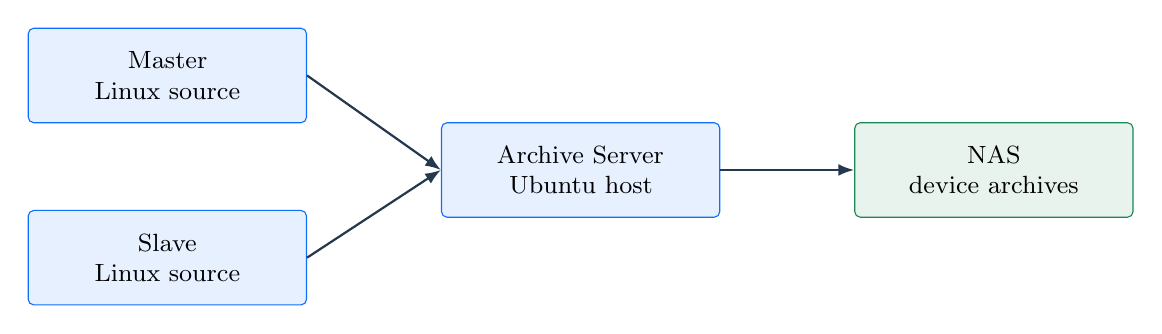
\begin{tikzpicture}[node distance=11mm and 17mm]
\node[primary](master){Master\\Linux source};
\node[primary,below=of master](slave){Slave\\Linux source};
\node[primary,right=of master,yshift=-12mm](server){Archive Server\\Ubuntu host};
\node[store,right=of server](nas){NAS\\device archives};
\draw[flow](master.east)--(server.west);\draw[flow](slave.east)--(server.west);
\draw[flow](server)--(nas);
\end{tikzpicture}\end{center}
The arrows describe the logical backup direction. The server initiates reads;
sources do not push to the NAS. Browsers connect to the archive host, which reads
the NAS and serves data. Source computers may be shut down after backup acceptance,
while the archive host and NAS remain available.

\section{Boundaries and guarantees}
\begin{itemize}
\item Device identities, archive data and imported Collections are separated.
\item Existing published raw runs are not overwritten. Changed runs become revisions.
\item New server analysis results are stored separately from raw backups.
\item No reverse synchronization writes server results into Master or Slave.
\item Source deletion does not delete a published NAS backup.
\item One transfer queue processes devices and runs sequentially. Checksum reads
within one run may use four workers.
\end{itemize}
\notetext{A NAS copy is not an independent disaster-recovery strategy by itself.
Arrange NAS snapshots, separate backups and retention with the laboratory's storage
administrator. The application does not configure those services.}

\chapter{Deployment and first initialization}
\section{Prepare the archive host}
Use a normal Linux account that owns the project checkout, its configuration and
SSH identity. Clone or pull the desired branch without sudo. Use a fixed or
reserved LAN IP for the host and source devices.
\begin{lstlisting}[language=bash]
cd /home/miga/MIGA-controller
git checkout marker-optimization
git pull --ff-only
./launch_code --archive
\end{lstlisting}
In LaunchUI choose \ui{Archive Server}. Use \ui{Check environment} and, if needed,
\ui{Repair environment}. Missing graphical or Linux prerequisites are installed
only after explicit approval in the terminal. Archive preparation must not start
the Controller hardware runtime.

\section{Mount the NAS permanently}
The application needs a local absolute filesystem path, for example
\pathcode{/mnt/miga-archive}. An address such as
\pathcode{smb://nas/share} is a file-manager connection, not the path expected by
the archive configuration. SMB/CIFS and NFS mounts are supported. Desktop GVFS/AFP
mounts are suitable only for exploratory tests, not unattended startup.
\begin{procedure}{Storage readiness}
\item Have the administrator configure the NAS export, credentials, account permissions
and persistent Linux mount. Do not put NAS credentials into Git or the web Guide.
\item Check the mount from the archive host using \code{findmnt /mnt/miga-archive}.
Confirm that the normal server account can read and write the dedicated backup folder.
\item Reboot and verify the mount again before enabling unattended server startup.
\item Keep sufficient free space for incoming data, immutable revisions and analyses.
\end{procedure}
\warningtext{Do not initialize an arbitrary existing data folder. Choose a dedicated
backup root. An absent network mount must not silently redirect backups into the
archive host's local disk. The server checks the archive identity marker and expected
filesystem before backup operations.}

\section{The five-step Guide}
\begin{longtable}{p{27mm}p{126mm}}\toprule
Step&Action and acceptance criterion\\\midrule\endhead
1. NAS&Select a detected mount or enter the dedicated backup root. Inspect it read-only;
confirm initialization or reuse only after reviewing the path, filesystem and space.\\
2. Devices&Register each source with a unique computer identity, role, host, Linux user
and absolute Data\_log path. Reuse existing registrations instead of duplicating them.\\
3. SSH and folders&Prepare the source locally, verify its host fingerprint, authorize
the server key, then use Test / discover to confirm access and locate Data\_log.\\
4. Verify backup&Perform the first full eligible-run pull, review the job, inspect
Collections and run a NAS checksum verification. This is not a small sample transfer.\\
5. Startup&Configure daily LaunchUI use or a systemd user service; test after reboot.\\
\bottomrule\end{longtable}
The Guide preserves existing configuration and does not replace keys or devices
automatically. Start opens the homepage; if storage is uninitialized, the homepage
redirects to the Guide. \ui{Open setup Guide} remains available for later checks.

\chapter{Sources and secure SSH pairing}
\section{Register the computer, not the username}
Master and Slave may both report \code{miga} from \code{whoami}. Their device IDs
must still differ, for example \code{master-22} and \code{slave-21}.
\begin{tabularx}{\textwidth}{p{37mm}X}\toprule
Field&Meaning\\\midrule
Device ID&Permanent archive namespace; lowercase letters, digits, dots, underscores or hyphens.\\
Display name&Human-readable name shown in the sidebar and device card.\\
Role&Master, slave or standalone; not an SSH authentication setting.\\
Host and SSH user&Source computer IP/hostname and its actual Linux account.\\
Data\_log path&Absolute source path, such as \pathcode{/home/miga/MIGA-controller/Data_log}.\\
Collection path&Optional explicit SQLite location; otherwise the Data\_log default is used.\\
SSH key path&Private identity on the archive host, not a path on the source computer.\\
\bottomrule\end{tabularx}

\section{Pair through LaunchUI}
\begin{procedure}{First pairing}
\item On the source, open \code{./launch_code --archive} and select
\ui{Prepare this source computer}, logged in as the data owner.
\item Choose Data\_log and use \ui{Prepare SSH / rsync}. Approve sudo locally if
installation or service preparation is needed. Optional recursive read/traverse ACL
repair is a separate confirmation, confined to the selected Data\_log.
\item Show the source host fingerprint. On the archive host select the registered
device, then \ui{Pair / reuse existing SSH}.
\item Compare the fingerprint independently. Enter only the matching
\code{SHA256:...} token, not the IP, key type or entire output line. A mismatch is
a reason to stop and investigate, not to disable verification.
\item Enter the source account password only in the native SSH terminal when asked.
The web application does not receive or save it. A working connection is reused.
\item Return to the Guide and use \ui{Test / discover}. Verify the selected data
directory and its read access before starting a full pull.
\end{procedure}
The default dedicated server identity is
\pathcode{~/.ssh/miga_archive_ed25519}. Existing keys and authorized-key entries
are preserved. Alternatively, the source LaunchUI can explicitly authorize the
server's public key. Never transfer the private key to a source.

\section{Device management}
\ui{Device management} provides registration, edit, enable/disable, connection
checks, manual pulls and removal. Removing a registration retains its NAS data and
analysis results. A device ID cannot be renamed. A source host/path change for an
already backed-up device requires a new identity rather than silently reassigning
the existing archive. Disable accidental duplicate sources before pulling.

\chapter{Daily operation and the dashboard}
\section{The homepage as a hub}
Open \pathcode{http://SERVER-IP:8765/}; the port is configurable in LaunchUI.
The English desktop-first homepage contains a compact NAS/device/job summary,
device cards, backup activity, recent records and a Server update panel. Tabler
styles are bundled locally for the dashboard and device-management pages.
\begin{itemize}
\item Sidebar device links and \ui{Open Archive} open the selected device Archive in
a new browser tab. The server homepage remains available as the hub.
\item \ui{Storage details} exposes the root path, mount, filesystem, free space,
identity check and inspection time. Storage inspection is cached for up to 15 seconds.
\item \ui{Connection \& backup details} shows the source, check time, last attempt,
publication job, Collection receipt and last checksum result.
\item Source connection checks are read-only and cached. A background check runs
every ten minutes when no backups are queued/running; this is separate from the
configurable backup interval. Old checks are labelled stale.
\end{itemize}
Dates use \code{dd/mm/yy HH:mm} in the browser's local timezone. An offline source
does not make already-published NAS archives unavailable.

\section{Manual pull procedures}
\begin{procedure}{One source}
\item Confirm the NAS is ready and the source is enabled.
\item Click \ui{Pull now} on the device card or management row and confirm the action.
\item Observe queued/running activity and the final record. Unchanged runs are skipped.
\end{procedure}
\begin{procedure}{All sources}
\item Click \ui{Pull all sources} on the homepage.
\item Review the inline confirmation, then choose \ui{Confirm pull all}.
\item Read the per-device results: queued, already queued, disabled or failed.
An existing queued/running job is not duplicated.
\item Follow the serial queue. An asynchronous source failure is recorded in that
source's job; the following devices are still processed.
\end{procedure}
Both actions leave saved automatic settings unchanged. A manual job nevertheless
becomes the most recent job used to calculate the next automatic due time.
NAS unavailability or reload maintenance blocks queue creation.

\section{Read the result correctly}
Published, unchanged and eligible counts do not measure all source directories:
deferred runs are excluded from eligible counts. A successful pull/check may publish
zero runs. Its timestamp means an eligible-set check completed without a task error
or failed run, not that new data necessarily arrived. SYNC warnings and deferred runs
can coexist with that successful check.

\chapter{Backup settings and scheduling}
\section{Global defaults and device overrides}
Open \ui{Backup settings}. Edit global values, expand a source and enable automatic
pulls as needed. Check \ui{Override} only for values that should differ from the
global defaults. For boolean overrides, the separate \ui{Enabled} checkbox is the
override value; an unchecked override means inheritance, not false.
\begin{longtable}{p{53mm}p{25mm}p{68mm}}\toprule
Setting&Default&Meaning\\\midrule\endhead
Pull interval&10 minutes&Normal automatic interval; configurable from 1 to 10080 minutes.\\
Pull on startup&Off&When enabled, the first scheduling check after startup may queue a pull; otherwise the initial interval is respected.\\
File quiet period&60 seconds&Minimum time since the newest run-file modification; allowed range 60--86400 seconds.\\
Initial failure retry&10 minutes&First failed-task retry delay; later consecutive failures double it.\\
Maximum failure retry&60 minutes&Upper bound for that exponential retry delay; cannot be below the initial delay.\\
Collections first&On&Take the source database snapshot before processing runs, rather than after the run loop.\\
\bottomrule\end{longtable}
Click \ui{Save backup settings}; review the success message. Settings are stored in
the archive host's configuration, not in raw run folders. Existing device automatic
switches are retained when upgrading. New jobs freeze their effective policy when
queued, so changes do not rewrite an already queued/running job's policy.

\section{Timing, queueing and retry}
The scheduler checks due times every five seconds. It does not transfer every five
seconds. One shared worker executes jobs sequentially, so a source's displayed next
time is a scheduling due time, not a completion guarantee. Queued/running devices
have no second due job. Disabled sources and sources with automatic pulls off have
no automatic due time.

Normal intervals are anchored to the most recent job start. A failed job, or one
with failed runs, uses the configured initial retry delay multiplied by powers of
two, capped at the maximum. A clean task result resets the failure streak. Deferred
and SYNC-only results do not trigger failure backoff. After restart, startup policy
also governs the first scheduling opportunity. NAS/queue rejections before a job
exists wait the initial retry delay in memory.
\notetext{A longer interval reduces scan frequency but increases the time until newly
completed runs become available. Every pull still inventories the source run tree;
there is no completion-event push or permanently incremental source index.}

\chapter{Eligibility, integrity and immutable publication}
\section{Which runs are eligible}
The source reader scans numeric year/month/day directories containing run folders.
A run needs \code{config.json}, \code{results.csv} and the configured quiet time.
Temporary files ending in \code{.tmp} or \code{.part} are excluded; symbolic links
are rejected rather than followed into other directories.

New-format runs use the existence of \code{archive_complete.json} as the completion
indicator. The reader does not validate the marker's JSON content. For legacy runs
without a marker, today's runs require the Controller status endpoint to confirm
the experiment is idle. Older-date runs may qualify without that idle confirmation
once the required files and quiet time are satisfied. Unready runs are deferred
for another scan.

\section{Incremental detection and verification}
The inventory fingerprint uses relative paths, sizes and nanosecond modification
times. A matching published receipt skips transfer and hashing. New/changed runs
are copied to incoming staging, followed by source SHA-256 calculation, source
stability checks and NAS SHA-256 verification. Only verified staging is published.
\begin{center}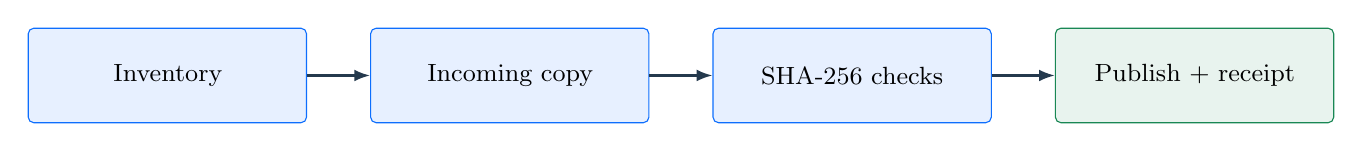
\begin{tikzpicture}[node distance=8mm]
\node[primary](scan){Inventory};
\node[primary,right=of scan](copy){Incoming copy};
\node[primary,right=of copy](check){SHA-256 checks};
\node[store,right=of check](publish){Publish + receipt};
\draw[flow](scan)--(copy);\draw[flow](copy)--(check);\draw[flow](check)--(publish);
\end{tikzpicture}\end{center}
\warningtext{Metadata-based skipping can miss a source edit that preserves both file
size and modification time. NAS verification compares files with saved receipts;
it does not re-read every unchanged source file to detect such an edit.}

\section{Changes, interruptions and verification}
A changed previously published run goes into a revision directory. Original run
files are not replaced. Transfers can retain partial staging across interruptions.
A file-list mismatch preserves staging in quarantine and requires a later retry.
Missing publication receipts can be recovered by validation instead of blindly
re-copying or overwriting data.

Use \ui{Verify checksums} in device details or the Guide to read all files referenced
by saved receipts. It may take a long time on a NAS. Review checked-file counts and
issues; zero checked files is not useful acceptance evidence. A saved successful
verification is a point-in-time result, not perpetual assurance.

On non-CIFS storage, published files/directories receive read-only permissions.
On CIFS/SMB, effective permissions depend on mount options; per-file chmod is not
used as the immutability mechanism. Application-level separation still prevents
analysis from overwriting raw backups. Administrators with filesystem write access
can modify data outside the application.

\chapter{SYNC, Collections and analysis}
\section{SYNC is not a transfer failure}
Master and Slave are backed up independently. A source
\code{sync_manifest.json} replication status other than complete is recorded as
a warning. Available eligible source data may still be backed up; the server does
not infer missing files from another source or block all devices until synchronization
is complete. Later source changes are discovered by the next inventory and stored
as revisions. A successful NAS checksum does not prove source SYNC completeness.

\section{Collection snapshots}
The source database is opened read-only and copied using SQLite's backup interface
to a temporary consistent snapshot. The server validates the snapshot and stores it
by content hash, then updates the latest-import pointer. The default is to do this
before the run loop; it can be configured to run afterwards. Snapshots can therefore
refer to runs that are not yet published or are deferred.

If the source database does not exist, the reader reports absence and does not
delete an earlier imported snapshot. If an early Collection snapshot fails, run
processing is still attempted, but the final job reports that Collection error.
During source downtime the last received snapshot remains available.

Imported \ui{Source Collections} are read-only. The archive host's own Collections
are separate and editable. Favourites and folders created on the server are not
written back to the Controller. A Collection receipt time indicates snapshot
receipt, not necessarily a user edit or a new database version.

\section{Use the full device Archive}
Open the desired device's Archive, choose Timeline or Collections, select a run
and load its data. Use the available metric, waveform, SYNC-node, analysis and
export controls as in the Controller Archive. Refer to the Controller manual for
the detailed scientific meaning of optimization and analysis parameters.

Server-side saves/reanalysis produce server-only analysis versions rather than
replacing original acquisition results. Review the selected source/device and
version before comparing or exporting results. A run directory in a revision store
must not be assumed to be the default Timeline selection: the implementation's
normal raw-run namespace remains distinct from revision and analysis stores.

\chapter{Updating, reloading and unattended operation}
\section{Server update panel}
\begin{procedure}{Select and apply an update}
\item Open the homepage locally through \pathcode{http://127.0.0.1:8765/},
or remotely using the archive host's address and port.
Remote clients can refresh branches, apply updates and configure or trigger reloads.
These operations require same-origin browser requests. The dashboard has no login;
provide access only to trusted clients through the network or an authenticated proxy.
\item Open \ui{Server update}. Review current checkout, repository source, local
changes and auto-reload preference.
\item Choose a branch from the dropdown. Selection previews cached remote metadata
without switching code or saving the selection.
\item Use \ui{Refresh Remote} to fetch known branches and save the chosen branch/source.
Only credential-free GitHub HTTPS or SSH repository URLs are accepted. Confirm any
repository-source change; use trusted code only.
\item Review remote commit/message, ahead/behind state and refresh time. Cached
metadata is not a live GitHub check. Local changes and divergent target history are
not overwritten, reset or stashed by the updater.
\item With backups idle, click \ui{Update Now} and confirm. Inspect pull output and
any errors. If auto reload is disabled, restart normally through LaunchUI afterwards.
\end{procedure}
Changing Git ownership or performing administrator repairs is not a web-update action.
The updater never uses sudo to fetch or pull.

\section{Safe reload}
In LaunchUI enable \ui{Auto reload after successful web update} to persist the
preference. Alternatively use \ui{Reload server safely} manually. This is explicit
graceful process replacement, not continuous file watching or a zero-downtime code swap.
Queued/running backups block it. New jobs are fenced while a reload is pending.

A detached helper waits for the old managed process to exit before starting a new
one. For systemd, a separate transient user unit requests the matching service's
restart, outside the server unit's cgroup. Unknown foreground processes are never
killed. No forced kill or duplicate server is used on timeout. Dashboard pages wait
for a different responding process ID, then refresh and report that new code is active.
Dependency changes may require \ui{Repair environment} before successful startup.

\section{Startup service and stopping}
\ui{Enable startup service} installs/enables a systemd user service for the current
project, configuration and port; an existing unit is preserved as a previous copy.
Installation does not stop a currently running foreground/detached server. Avoid
running two processes against the same configuration. \ui{Enable before-login startup}
uses an explicitly approved sudo action to enable linger for the normal Linux user.
\begin{lstlisting}[language=bash]
systemctl --user status miga-archive.service --no-pager
journalctl --user -u miga-archive.service -n 150 --no-pager
\end{lstlisting}
\ui{Stop gracefully} sends one shutdown request. Allow the current run to finish;
do not send repeated signals or start another process while stopping. Closing
LaunchUI does not stop a detached server. Unexpected restarts mark unfinished jobs
interrupted; a later manual or automatic pull can resume retained staging.

\chapter{Troubleshooting and acceptance}
\section{Common symptoms}
\begin{longtable}{p{41mm}p{112mm}}\toprule
Symptom&Interpretation and safe next step\\\midrule\endhead
Source offline&Existing NAS archives remain accessible. Check source power, IP,
SSH service and account access. Automatic failures follow retry backoff.\\
Source check stale&The cached connection check is old or configuration changed.
Use Check source; do not assume the displayed cached success proves current access.\\
Job incomplete&Inspect failed, deferred and SYNC-warning lists separately. It is
not synonymous with a failed NAS transfer.\\
No new runs&Check eligible/deferred counts, quiet time, completion marker and, for
today's legacy runs, Controller idle-status access.\\
Slow first backup&Full inventory, many files, network transfer and SHA-256 reads
take time. Watch phase/counts. Do not disable integrity checks to improve speed.\\
NAS unavailable&Verify permanent mount, archive identity, expected filesystem,
permissions and free space. Do not initialize an empty local substitute.\\
Checksum issues&Preserve receipts and affected data; investigate storage/source
state. Do not delete originals or quarantine as a first response.\\
Update permission error&Inspect checkout and Git object ownership as the normal
server user. Do not use sudo git or chmod 777.\\
Reload failed&Inspect reload state/log or user-service journal. Check whether the old
process is stopping or the new one failed before issuing another start.\\
\bottomrule\end{longtable}

\section{Diagnose Git ownership}
Run diagnostics in the archive host checkout, not on Master or Slave:
\begin{lstlisting}[language=bash]
whoami
pwd
ls -ld .git .git/objects
find .git/objects -maxdepth 2 ! -user "$(whoami)" -ls | head -20
\end{lstlisting}
Root-owned objects commonly result from earlier sudo Git commands. After verifying
the exact checkout, account and intended ownership, an administrator can repair
only that repository's Git metadata. For the documented example, not a universal command:
\begin{lstlisting}[language=bash]
sudo chown -R miga:miga /home/miga/MIGA-controller/.git
\end{lstlisting}
Do not recursively chown the NAS, home directory or an unrelated repository.
If code files also have wrong ownership, inspect their exact paths separately.

\section{Before shutting sources down for a month}
\begin{enumerate}
\item Pull all enabled sources and wait for every relevant job to finish.
\item Resolve failed transfers; separately review deferred runs and source SYNC warnings.
\item Verify checksums and review checked-file counts and issues for each device.
\item Open representative old/new runs and both source/own Collections in each Archive.
\item Confirm source shutdown does not prevent NAS-backed browsing from another terminal.
\item Reboot-test the archive host, NAS mount and startup service; preserve configuration,
keys, receipts, logs and the independent NAS backup/snapshot strategy.
\end{enumerate}

\appendix
\chapter{Paths, interfaces and operator reference}
\begin{longtable}{p{57mm}p{96mm}}\toprule
Location&Purpose\\\midrule\endhead
\pathcode{~/.config/miga-archive/config.json}&Default local configuration; can be overridden with \code{MIGA_ARCHIVE_CONFIG}.\\
Configuration sibling \code{jobs/}&Persisted job records and effective policies.\\
Configuration sibling \code{launcher/}&Runtime/preferences, server/reload logs and reload state.\\
NAS \code{incoming/}&Partial staging; not accepted published data.\\
NAS \code{quarantine/}&Preserved mismatched staging for investigation.\\
NAS \code{devices/DEVICE/runs/}&Original device-separated published runs.\\
NAS \code{devices/DEVICE/revisions/}&Changed-run versions; originals remain.\\
NAS \code{devices/DEVICE/state/}&Receipts and integrity verification results.\\
NAS \code{devices/DEVICE/collection-imports/}&Immutable source Collection snapshots and latest pointer.\\
\bottomrule\end{longtable}
Use the UI as the normal interface. \pathcode{/devices} is device management,
\pathcode{/backup-settings} is backup policy, and \pathcode{/setup} resumes the Guide.
\pathcode{/archive-server/backup-all} queues the enabled-source batch.
\pathcode{/archive-server/backup-settings} reads/saves policy through the appropriate
GET/PUT method. Device Archive URLs include the device ID and are not interchangeable.

Implementation reference: \pathcode{archive_main.py},
\pathcode{app/archive/backup.py}, \pathcode{app/archive/backup_policy.py},
\pathcode{app/archive/remote_reader.py}, \pathcode{app/archive/configuration.py},
\pathcode{app/archive/updater.py}, \pathcode{app/archive/reload.py},
\pathcode{app/archive/launcher_runtime.py} and \pathcode{app/archive/launcher_ui.py}.

\backmatter
\chapter*{Revision note}\addcontentsline{toc}{chapter}{Revision note}
Prepared on \documentdate{} against \commitid{}. This revision documents configurable
backup policy, Collections-first pulls, Pull all sources, full branch-aware updates,
safe automatic reload and the desktop dashboard. Screenshots are deliberately not
required to compile this standalone source; diagrams, tables and operating procedures
remain reproducible without external image assets. Future code changes should be
reviewed against this revision before updating operator instructions.
\end{document}
